\section{Time box 4}
\listoftodos
\subsection{Time box planning}
\begin{figure}[H]
	\begin{centering}
		\missingfigure{Updated timebox figure}
		%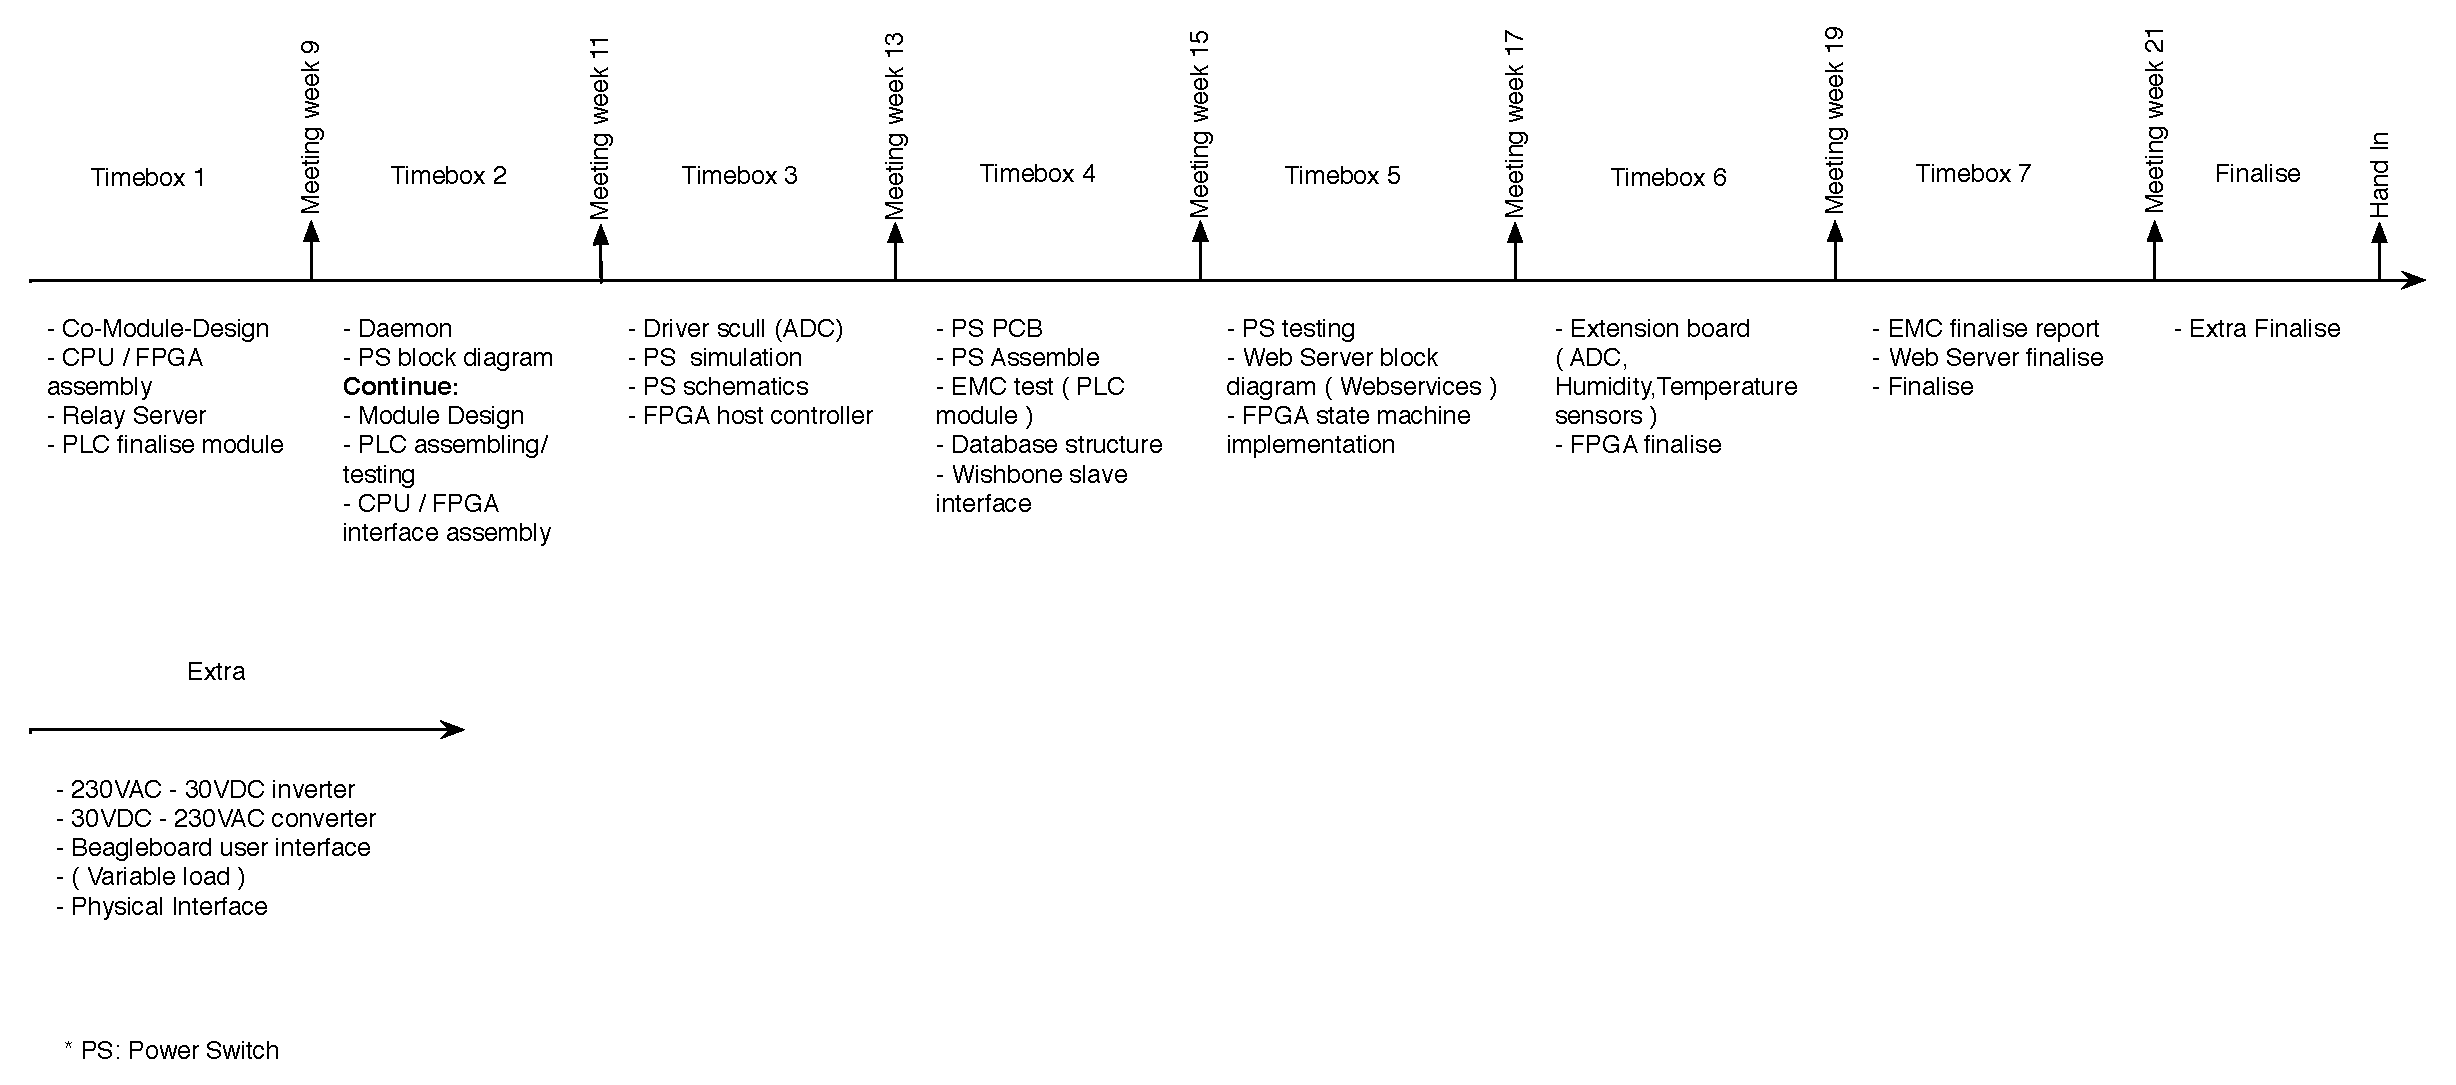
\includegraphics[width=1.0\textwidth]{images/tb_r3.pdf}
		%\caption{Updated time-box}
	\end{centering}
\end{figure}
\subsubsection{Work to be done in this time box}
\begin{itemize}
	\item Power line communication module
	\begin{itemize}
		\item EMC test of modules
	\end{itemize}
	\item Database
	\begin{itemize}
		\item \todo[author=Jesus, inline]{edit what you like and bake a cake}
	\end{itemize}
	\item Physical interface
	\begin{itemize}
		\item Wishbone slave interface
		\item Switch driver
		\item LED driver
	\end{itemize}
\end{itemize}
\paragraph{Description:}
\begin{description}
	\item[Power line module] \todo[author=Dennis, inline]{edit here Dennis}
	\item[Database] \todo[author=Jesus, inline]{edit here Jesus}
	\item[Physical interface] is the light indication and the switches that shall be on the physical hub interface
\end{description}
\subsubsection{Time planning}
\begin{table}[H]
\centering
	\begin{tabular}{|l|c|c|c|c|}
		\hline
		~			& PLC module	& Database	& Physical interface\\ \hline
		Estimation	& xx			& 10		& 12				\\
		Actual		& xx			& xx		& xx				\\
		Developer	& Dennis		& Paulo		& Theis				\\
		\hline
	\end{tabular}
	\caption{Estimation and actual time used on the project}
\end{table}
\subsection{Power line communication module - Dennis}
%			intro
%			
%					verification specification
%					deployment specification
%					
%			Analysis
%	
%	                Refactored block diagram
%	                Refactored class diagram
%	                Detailed use cases
%	                User interface specification
%	                System interface specification
%	                Dimensioning specification 
%	
%	        Design
%	
%	                UML/SysML deployment view(s)
%	                Mechanical specifications and dimensioning
%	                HW module specification per block
%	                UML SW deployment view
%	                Class specification
%	                Refactored class diagram
%	                Use case scenarios specifications
%	                Sequence diagrams 
%	
%	        Implementation
%	
%	                Mechanical drawings with details explained
%	                Electronic diagrams with details explained
%	                Source code with details explained
%	                Description of integration 
%	
%	        Verification
%	
%	                Module tests
%	                Integration tests
%	                Acceptance test
\subsection{Database - Paulo}
%		Intro

Each module of the system has sensors and data to be stored and shown to the user. As such, data have to be stored in a convenient and consistent way. A SQL database ( MySQL) is used. All data stored have to be present in a web interface the integration between this type of data base and a server-side scripting ( PHP ) keeps the development faster and completely open source.
A database have to be consistent, flexible and efficient so no data is lost or repeated when a value is send to it.
%
%			Verification specification
\subsubsection{Verification specification}
A LAMP ( Linux Apache MySQL PHP ) web server is implemented at the development environment used to build the uClinux image. This use a linux distribution Centos virtual machine in which the web server was built ( how to build the web server explanation further in this documentation ).
For an easy and fast verification and development of the database a phpMyAdmin web application was installed at the server.
The verifications can be found at the end of this section.

%			Deployment specification
\subsubsection{Deployment specification}
\missingfigure{Have no idea what this should be}

%		Analysis
%	
%	                Refactored block diagram
%	                Refactored class diagram
%	                Detailed use cases
%	                User interface specification
%	                System interface specification
%	                Dimensioning specification 
\subsubsection{Analysis}
To develop a database, data models are generated from the requirements and system information analysis, this is an abstract way of presenting the data to be stored.
\paragraph{Requirements}
	\begin{itemize}
		\item Jan is looking at the web interface for the energy hub. From where he can see the status for each modules connected to it
in a graphically way.
		\item A new energy module is connected to the hub, Jan opens the web interface for the energy hub, he logs in the administrator section of the system
to start, stop or see a more detailed overview of each module.
		\item Jan arrives at the university in the morning and an email was send to him reporting a failure in the green energy system, he login to the administrator web interface, and he can see what the problem might be, and if it's possible to solve it directly on the interface.
	\end{itemize}

From this requirements given by the customer the relevant information for the database development is filtered:
	\begin{itemize}
		\item The status of each module have to be show.
		\item A detailed overview of each module such as current production (Voltage, Current, Power, etc.), efficiency of the module, etc.
		\item Errors have to be reported to the system administrator / maintainer.
	\end{itemize}
	
In a deeper analysis of the information system for the power energy hub, some technical data is needed to be stored such as:
	\begin{itemize}
		\item Each module have is unique id, this is similar to the MAC address, this way when a module is connected is possible to check if the module have been connected before, so the data can be stored for the same module instead of instantiate a new module which can generate ambiguous data.
		\item Three types of modules are defined: input, output and bidirectional. This are seen from the power hub point of view where inputs are producers ( solar panels, wind turbine, ... ), output are consumers ( Inverter, 30V output socket ) and bidirectional ( C.A.E.S, batteries, ...).
	\end{itemize}

%	        Design
%	
%	                UML/SysML deployment view(s)
%	                Mechanical specifications and dimensioning
%	                HW module specification per block
%	                UML SW deployment view
%	                Class specification
%	                Refactored class diagram
%	                Use case scenarios specifications
%	                Sequence diagrams 
%	
\subsubsection{Design}

\paragraph{Data sets}

From the system information analysis a basic tabular structure is designed for a better understanding and overview of the data, this is called data set structure.
\\\\
TYPE(ID\_TYPE, TYPE);

\begin{table}[H]
\centering
	\begin{tabular}{| p{2cm} | p{10cm} |}
		\hline
		ID\_TYPE & Auto increment integer, a new id number is generated when a different type is needed to the system. \\\hline
		TYPE & Describe the type name for example: Input, output, bidirectional, etc.\\\hline
	\end{tabular}
\end{table}

STATUS(ID\_STATUS, STATUS);

\begin{table}[H]
\centering
	\begin{tabular}{| p{2cm} | p{10cm} |}
		\hline
		ID\_STATUS & Auto increment integer, a new id number is generated when a different status is needed to the system. \\\hline
		STATUS & Describe the status name for example: Running, stopped, warning, etc.\\\hline
	\end{tabular}
\end{table}


MODULES(ID\_MODULE, UNIQUE\_ID, ID\_TYPE, ID\_STATUS, NAME);

\begin{table}[H]
\centering
	\begin{tabular}{| p{2cm} | p{10cm} |}
		\hline
		ID\_MODULE & Auto increment integer, a new id number is generated every time an unknown module is connected. \\\hline
		UNIQUE\_ID & Module unique ID, this id as primary key ensures that no module with is repeated in the database.\\\hline
		ID\_TYPE & This is a foreigner key for the table type, this way if some other type of module is needed it can be dynamical add. \\\hline
		ID\_STATUS & This is a foreigner key for the table status, this way if some other status to the module is needed it can be dynamical add. \\\hline
		NAME & The name of the module for example, Solar Panel, wind turbine, battery. \\\hline
	\end{tabular}
\end{table}
As a requirement the database have to store the measurement  from different modules, the common and minimal measurements needed from the modules are current and voltage. So a log data set is created.
\\\\
LOGS(ID\_LOG, ID\_MODULE, DATE\_TIME, PORT, CURRENT, VOLTAGE);

\begin{table}[H]
\centering
	\begin{tabular}{| p{2cm} | p{10cm} |}
		\hline
		ID\_LOG & Auto increment integer, a new id number is generated every time an measurement is add. \\\hline
		ID\_MODULE & This is a foreigner key for the table modules, this allow the system to know from which module correspond the measurement .\\\hline
		DATE\_TIME & Date and time of the measurement is saved so it can be plotted or in case of a lower efficiency a detailed history can analysed. \\\hline
		PORT & Defines in which port or the energy hub the module is connected in the time of the measurement. \\\hline
		CURRENT & Current measurement. \\\hline
		VOLTAGE & Voltage measurement. \\\hline
	\end{tabular}
\end{table}

At this point the database can initialise a new module or identified if the module where connected before, change the status for each module and add new measurements for each module. ( Verification 1, 2 and 3 )

Measurements are add to the database every \todo{Time between measurements}, which in a non-stop system database size could be a problem, to avoid this situation a wrapper data set is created. This will store an average of values between a time span for each module, allowing the customer either to erase the values from the log or export them out from the database. Crucial data can be lost in this step for example the port history in case of troubleshooting, and precise date and time which would not allow the precise plot of data. 

WRAPPER(ID\_WRAP, ID\_MODULE, DATE\_FROM, DATE\_TO, AVG\_CURRENT, AVG\_VOLTAGE);

\begin{table}[H]
\centering
	\begin{tabular}{| p{2cm} | p{10cm} |}
		\hline
		ID\_WRAP & Auto increment integer, a new id number is generated every time an wrap is needed. \\\hline
		ID\_MODULE & This is a foreigner key for the table modules, this allow the system to know from which module correspond the values .\\\hline
		DATE\_FROM & Date and time of the time span start. \\\hline
		DATE\_TO & Date and time of the time span end. \\\hline
		AVG\_CURRENT & Average current measurements. \\\hline
		AVG\_VOLTAGE & Average voltage measurements. \\\hline
	\end{tabular}
\end{table}

The system is now able to decrease the amount of space needed using a time span and average values. ( Verification 4 )

During the verification process some problems related to the flexibility of the database were found:
	\begin{itemize}
		\item Problem 1: The Photovoltaic and Wind Turbine modules have more measurements to be stored then only current and voltage, for example velocity and direction of the wind, sun position, etc.
		\item \todo{Meeting with martin anytime this week to talk about the database structure}
	\end{itemize}

\paragraph{Problem 1}
In the design of this database it was assumed that all the modules would only save to the database the current and voltage. But during the verification process, the designed database was not flexible enough by the type of measurements being restrict to only current and voltage.

	\begin{itemize}
		\item How to make the database more flexible so it would allow inserting different measurements for different modules?
	\end{itemize}

Different approaches were made:
	
	\begin{itemize}
		\item Option 1: Create a new table for each new module that have extra measurements and add the ID\_EXTRA to the logs table.
		\item Option 2: Give different unique ids to the sensors and relate them to their modules, so the log will store the sensor measurement.
	\end{itemize}

Option 1 was not consistent since that every time a new module was connected a new table had to be created for that module with the needed measurement units.\\\\
Option 2 is the most reliable and the implemented one. A table Units and Sensors were created:\\
\\
SENSOR(ID\_SENSOR, ID\_MODULE, ID\_UNITS);

\begin{table}[H]
\centering
	\begin{tabular}{| p{2cm} | p{10cm} |}
		\hline
		ID\_SENSOR & Auto increment integer, a new id number is generated when a different sensor is needed to the system. \\\hline
		ID\_MODULE & This is a foreigner key for the table sensors, this allow the system to know from which module correspond the sensor, being a primary key with the id\_sensor, this way each sensor correspond to only one module .\\\hline
		ID\_UNITS & This is a foreigner key for the table units, this allow the system to know which units the sensor is measuring.\\\hline
	\end{tabular}
\end{table}

UNITS(ID\_UNIT, UNIT);

\begin{table}[H]
\centering
	\begin{tabular}{| p{2cm} | p{10cm} |}
		\hline
		ID\_UNIT & Auto increment integer, a new id number is generated when a different unit is needed to the system. \\\hline
		UNIT & Describe the unit name for example: A, V, deg ,m/s,etc. (Ampere, Volt, Degrees, Velocity)\\\hline
	\end{tabular}
\end{table}

In table wrapper and logs the ID\_MODULE was replaced with ID\_SENSOR. The database becomes more flexible since at anytime a module with new unknown sensors can be add and a sensor can be added to a existent module and the values will always be saved and retrieved to the user with the appropriat measurement units.

\paragraph{Data Model}


\begin{figure}[H]
	\begin{centering}
		%\missingfigure{Updated timebox figure}
		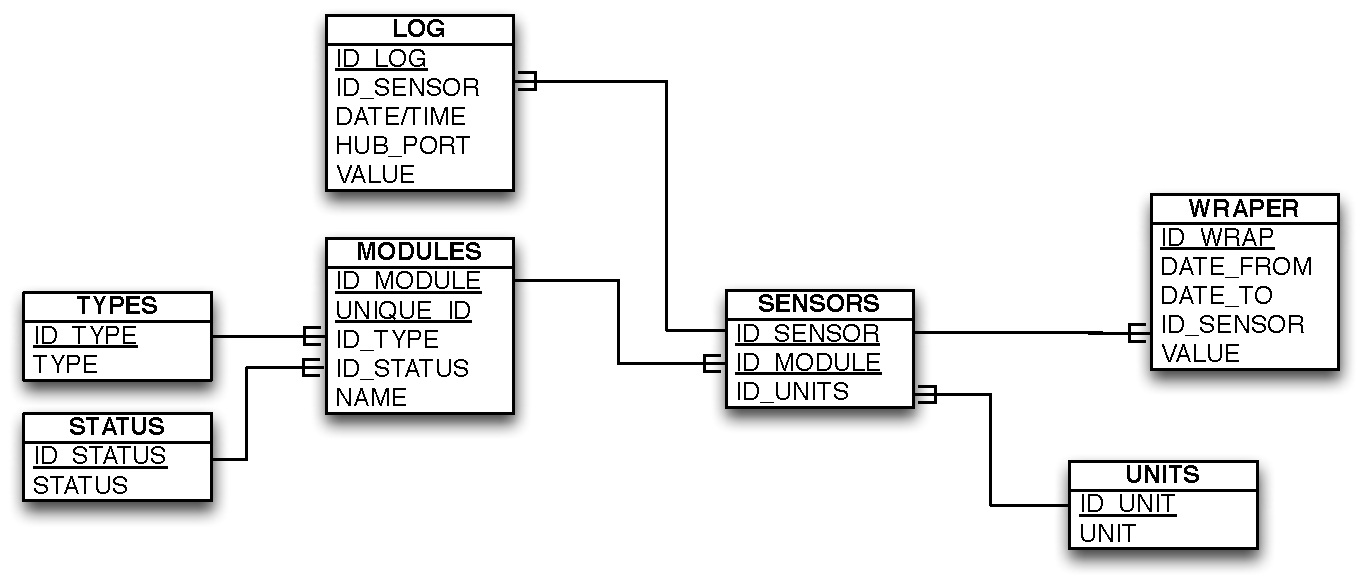
\includegraphics[width=1.0\textwidth]{images/db_structure.pdf}
		\caption{Data Model}
	\end{centering}
\end{figure}


%	        Implementation
%	
%	                Mechanical drawings with details explained
%	                Electronic diagrams with details explained
%	                Source code with details explained
%	                Description of integration 
%	
\subsubsection{Implementation}

%	        Verification
%	
%	                Module tests
%	                Integration tests
%	                Acceptance test
\subsubsection{Verification}
\begin{table}[H]
\centering
	\begin{tabular}{| c | l | c |}
		\hline
		Verification & Description & Acceptance \\\hline
		1 & Initialise a new module or identified if the module where connected before & ~ \\\hline
		2 & Change the status for each module & ~ \\\hline
		3 & Add new measurements for each module & ~ \\\hline
		4 & Decrease the database size using a time span and average values. & ~ \\\hline
		2 & Change the status for each module & ~ \\\hline
		2 & Change the status for each module & ~ \\\hline
		2 & Change the status for each module & ~ \\\hline
		2 & Change the status for each module & ~ \\\hline
		2 & Change the status for each module & ~ \\\hline
	\end{tabular}
\end{table}

\subsection{Physical interface - Theis}
%			intro
%			
%					verification specification
%					deployment specification
%					
%			Analysis
%	
%	                Refactored block diagram
%	                Refactored class diagram
%	                Detailed use cases
%	                User interface specification
%	                System interface specification
%	                Dimensioning specification 
%	
%	        Design
%	
%	                UML/SysML deployment view(s)
%	                Mechanical specifications and dimensioning
%	                HW module specification per block
%	                UML SW deployment view
%	                Class specification
%	                Refactored class diagram
%	                Use case scenarios specifications
%	                Sequence diagrams 
%	
%	        Implementation
%	
%	                Mechanical drawings with details explained
%	                Electronic diagrams with details explained
%	                Source code with details explained
%	                Description of integration 
%	
%	        Verification
%	
%	                Module tests
%	                Integration tests
%	                Acceptance test